\seminar{Encoding Exercises II}{12:00}{10/10/24}{Asim Ali}

\begin{minipage}[c]{0.47\linewidth}
  \begin{figure}[H]
    \centering
    \begin{tikzpicture}[scale=0.9]
      \draw[step=1cm,gray,very thin,dashed] (0.01,-0.99) grid (7.99,0.99);
      \draw (0,0) -- (8,0);
      \draw (0,-1) -- (0,1);
      \node at (0.5,1.25) {$1$}; \node at (1.5,1.25) {$1$}; \node at (2.5,1.25) {$0$}; \node at (3.5,1.25) {$0$};
      \node at (4.5,1.25) {$0$}; \node at (5.5,1.25) {$0$}; \node at (6.5,1.25) {$1$}; \node at (7.5,1.25) {$1$};
    
      \draw[thick,myPurple] plot[domain=0:4*pi, samples=60] ({(\x/pi)/2},{sin(\x r)});
      \draw[thick,myPurple] plot[domain=8*pi:24*pi, samples=120] ({(\x/pi)/4},{sin(\x r)});
      \draw[thick,myPurple] plot[domain=12*pi:16*pi, samples=60] ({(\x/pi)/2},{sin(\x r)});
    \end{tikzpicture}
    \caption{BFSK representation of the binary number $11000011$}
  \end{figure}
\end{minipage}\hfill
\begin{minipage}{0.47\linewidth}
  \begin{figure}[H]
    \centering
    \begin{tikzpicture}[scale=0.9]
      \draw[step=1cm,gray,very thin,dashed] (0.01,-0.99) grid (7.99,0.99);
      \draw (0,0) -- (8,0);
      \draw (0,-1) -- (0,1);
      \node at (0.5,1.25) {$1$}; \node at (1.5,1.25) {$1$}; \node at (2.5,1.25) {$0$}; \node at (3.5,1.25) {$0$};
      \node at (4.5,1.25) {$0$}; \node at (5.5,1.25) {$0$}; \node at (6.5,1.25) {$1$}; \node at (7.5,1.25) {$1$};
    
      \draw[thick,myPurple] plot[domain=0:4*pi, samples=60] ({(\x/pi)/2},{sin((\x - pi )r)});
      \draw[thick,myPurple] plot[domain=4*pi:12*pi, samples=120] ({(\x/pi)/2},{sin(\x r)});
      \draw[thick,myPurple] plot[domain=12*pi:16*pi, samples=60] ({(\x/pi)/2},{sin((\x - pi )r)});
    \end{tikzpicture}
    \caption{BPSK representation of the binary number $11000011$}
  \end{figure}
\end{minipage}

\begin{minipage}[c]{0.47\linewidth}
  \begin{figure}[H]
    \centering
    \begin{tikzpicture}[scale=0.9]
      \draw[step=1cm,gray,very thin,dashed] (0.01,-0.99) grid (7.99,0.99);
      \draw (0,0) -- (8,0);
      \draw (0,-1) -- (0,1);
      \node at (0.5,1.25) {$1$}; \node at (1.5,1.25) {$1$}; \node at (2.5,1.25) {$0$}; \node at (3.5,1.25) {$0$};
      \node at (4.5,1.25) {$0$}; \node at (5.5,1.25) {$0$}; \node at (6.5,1.25) {$1$}; \node at (7.5,1.25) {$1$};
    
      \draw[thick,myPurple] plot[domain=0:2*pi, samples=30] ({(\x/pi)/2},{sin((\x - pi)r)});
      \draw[thick,myPurple] plot[domain=2*pi:4*pi, samples=30] ({(\x/pi)/2},{sin((\x)r)});
      \draw[thick,myPurple] plot[domain=4*pi:12*pi, samples=120] ({(\x/pi)/2},{sin((\x)r)});
      \draw[thick,myPurple] plot[domain=12*pi:14*pi, samples=30] ({(\x/pi)/2},{sin((\x - pi)r)});
      \draw[thick,myPurple] plot[domain=14*pi:16*pi, samples=30] ({(\x/pi)/2},{sin((\x)r)});
    \end{tikzpicture}
    \caption{DPSK representation of the binary number $11000011$}
  \end{figure}
\end{minipage}\hfill
\begin{minipage}{0.47\linewidth}
  \begin{figure}[H]
    \centering
    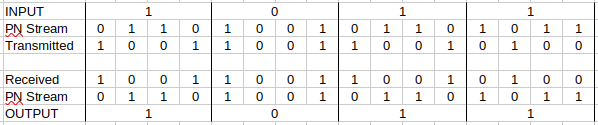
\includegraphics[width=0.99\linewidth]{assets/sem2-ex3.png}
    \caption{DSSS encoding and decoding of the binary number $1001$}
  \end{figure}
\end{minipage}